\section{Experiments}
\label{sec:exp}

\subsection{E0: $\alpha$ profile of the pretrained model}
\begin{figure}[t]
\centering
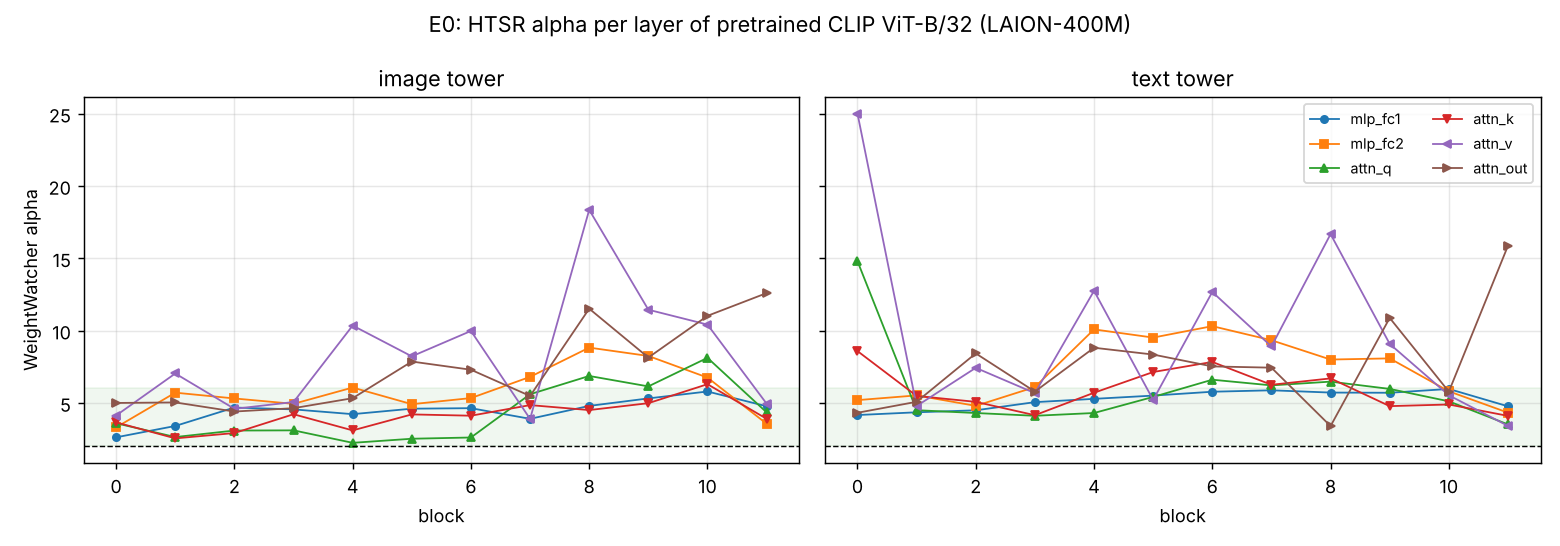
\includegraphics[width=\linewidth]{fig/e0_alpha_profile.png}
\caption{HTSR $\alpha$ per layer and role of the pretrained CLIP ViT-B/32 (LAION-400M). Shaded band: $2 < \alpha < 6$. No layer is below 2; attention value/output projections and late MLP output projections are ``under-trained'' by the HTSR reading.}
\label{fig:e0}
\end{figure}
WeightWatcher analysed all 148 matrices (Fig.~\ref{fig:e0}). No layer has $\alpha < 2$ (minimum 2.24); the model-wide mean is 6.3 and the median 5.5. Well-trained layers ($2<\alpha<5$) are the MLP input projections, the $q/k$ projections of the first six image blocks and the last block's output projection ($\alpha = 3.56$ with 459 eigenvalues beyond the Marchenko--Pastur bulk); $v$ and output projections of attention sit at 5--18. Image-tower $\alpha_{\mathrm{fc1}}$ rises almost monotonically with depth (2.6 at block 0 to 5.8 at block 10), so in this model ``closest to 2'' is confounded with ``early'', which is why E2b includes depth and random orders.

\subsection{E2a: single-block conversion damage versus $\alpha$}
\begin{figure}[t]
\centering
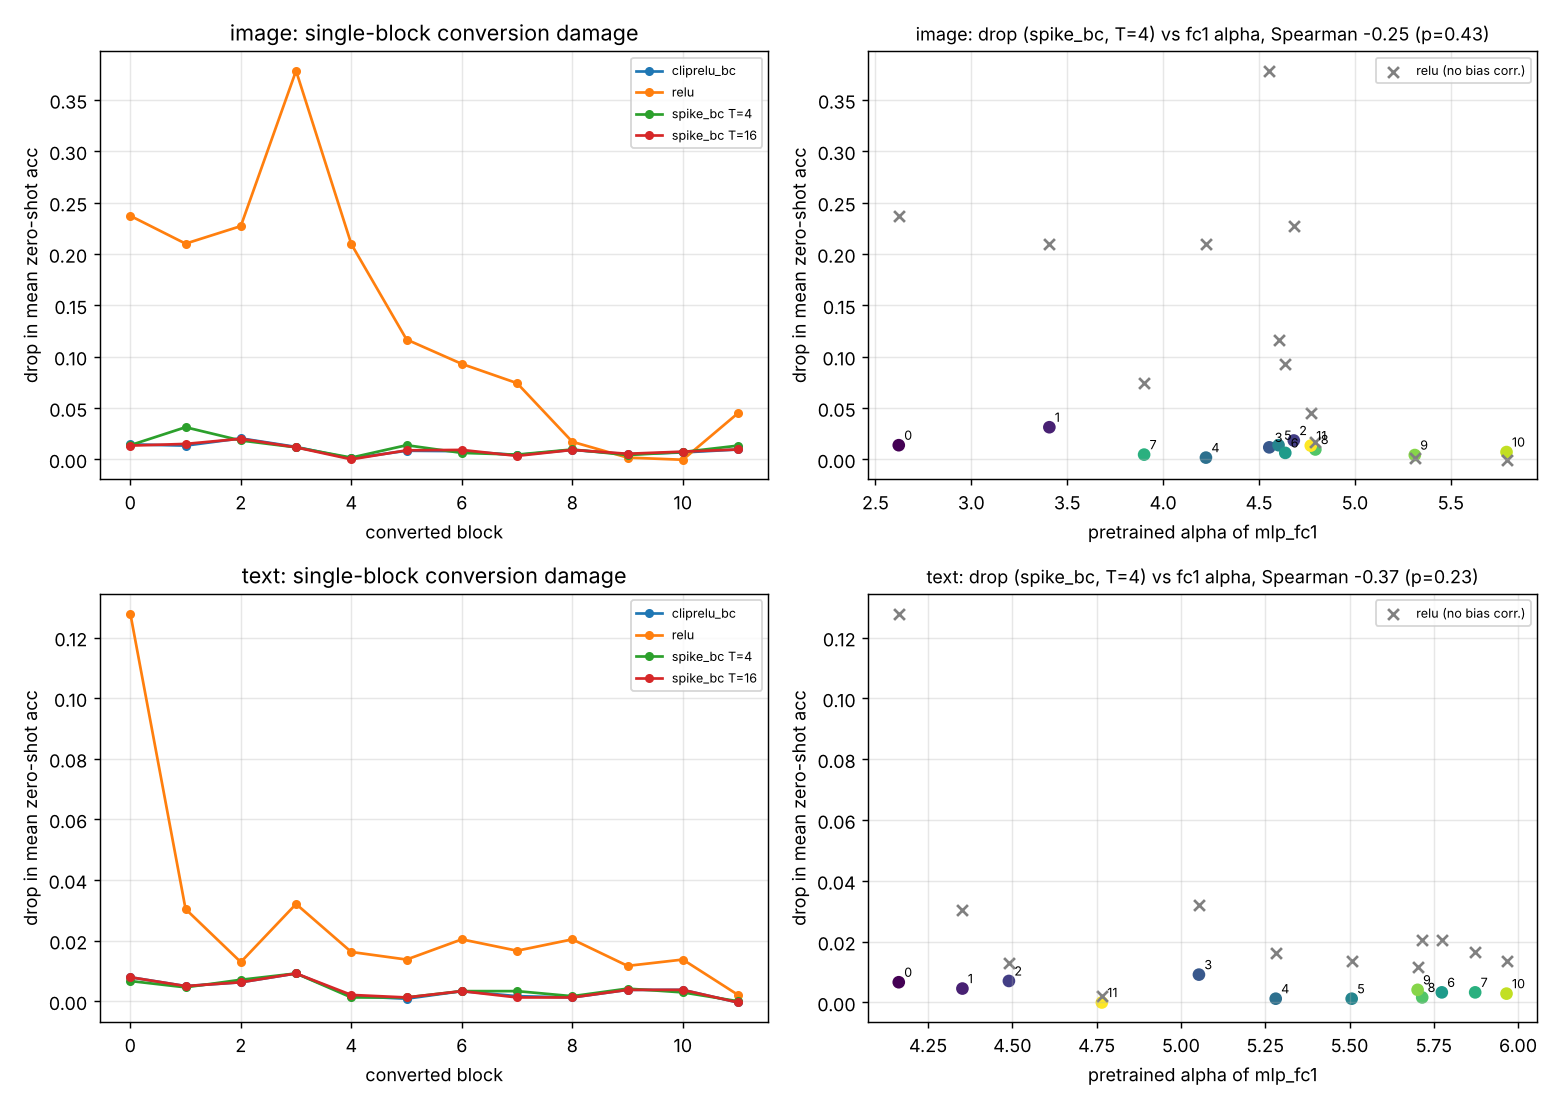
\includegraphics[width=\linewidth]{fig/e2a_damage_vs_alpha.png}
\caption{E2a. Left: drop in mean zero-shot accuracy when the MLP activation of one block is converted (ReLU rate code without correction; clipped ReLU and spiking populations at $T{=}4$ and $16$ with per-channel thresholds and bias correction). Right: the same drop against the block's pretrained $\alpha_{\mathrm{fc1}}$ (crosses: uncorrected ReLU).}
\label{fig:e2a}
\end{figure}
Figure~\ref{fig:e2a} and Tab.~\ref{tab:e2a} summarise 96 configurations. Without bias correction a single early image block costs 21--38 points and text block 0 costs 13; with per-channel thresholds and bias correction every block costs at most 2 points (image mean 1.1 at $T{=}4$, 0.9 at $T{=}16$ and in the clipped-ReLU limit; text mean 0.4), so the spike quantisation itself is worth 0.1--0.2 points and the GELU negative lobe is the whole story.

Does $\alpha$ predict the damage? In the image tower the \emph{sign is opposite to H2}: the blocks whose MLP $\alpha$ is closest to 2 (blocks 0, 1, 7, $\alpha_{\mathrm{fc1}}=2.6, 3.4, 3.9$) are the most damaged, strongly without correction (Spearman $-0.75$ with $\alpha_{\mathrm{fc1}}$, $-0.90$ with $\hat\alpha$, $p<0.01$) and weakly with it ($-0.59$ with $\alpha_{\mathrm{fc2}}$, $p=0.04$; $-0.25$ with $\alpha_{\mathrm{fc1}}$, n.s.). ``Well-trained'' by the HTSR reading means ``carries the signal'', and the signal is what a lossy activation destroys; the relation is confounded with depth and with the MLP's share of the block output (0.7--0.8 in blocks 0--7, 0.3--0.4 in blocks 8--10). In the text tower $\alpha$ does not predict damage ($|\rho|\le0.44$, $p>0.15$); the fc1 log spectral norm does weakly ($+0.54$ to $+0.60$, $p\approx0.05$). Retrieval is damaged in different places from classification: converting text block 0 or 1 costs 18 / 10 points of COCO R@1 against 0.5--0.8 points of accuracy, and the last image block costs 6 points of R@1.

\begin{table}[t]
\centering
\small
\begin{tabular}{lcccccc}
\toprule
 & \multicolumn{3}{c}{image tower} & \multicolumn{3}{c}{text tower} \\
predictor of drop & ReLU & spk$_4$ & spk$_{16}$ & ReLU & spk$_4$ & spk$_{16}$ \\
\midrule
$\alpha_{\mathrm{fc1}}$ & $-.75^{*}$ & $-.25$ & $-.20$ & $-.23$ & $-.37$ & $-.44$ \\
$\alpha_{\mathrm{fc2}}$ & $-.62^{*}$ & $-.59^{*}$ & $-.53$ & $+.13$ & $-.28$ & $-.30$ \\
$\hat\alpha_{\mathrm{fc1}}$ & $-.90^{*}$ & $-.43$ & $-.42$ & $+.35$ & $-.04$ & $-.18$ \\
$\log\|W_{\mathrm{fc1}}\|_2$ & $-.54$ & $-.29$ & $-.27$ & $+.60^{*}$ & $+.56$ & $+.57$ \\
frac.\ positive pre-act. & $+.72^{*}$ & $+.42$ & $+.34$ & $-.48$ & $-.49$ & $-.46$ \\
\midrule
mean drop (points) & 13.4 & 1.1 & 0.9 & 2.7 & 0.4 & 0.4 \\
\bottomrule
\end{tabular}
\caption{E2a: Spearman correlation across the 12 blocks of a tower between the single-block conversion damage (drop in mean zero-shot accuracy) and pretrained weight statistics; $^{*}$: $p<0.05$. $\hat\alpha$ is WeightWatcher's alpha-weighted; spk$_T$: spiking population with bias correction.}
\label{tab:e2a}
\end{table}
\subsection{E1: $\alpha$ during fine-tuning of an insert}
\begin{figure}[t]
\centering
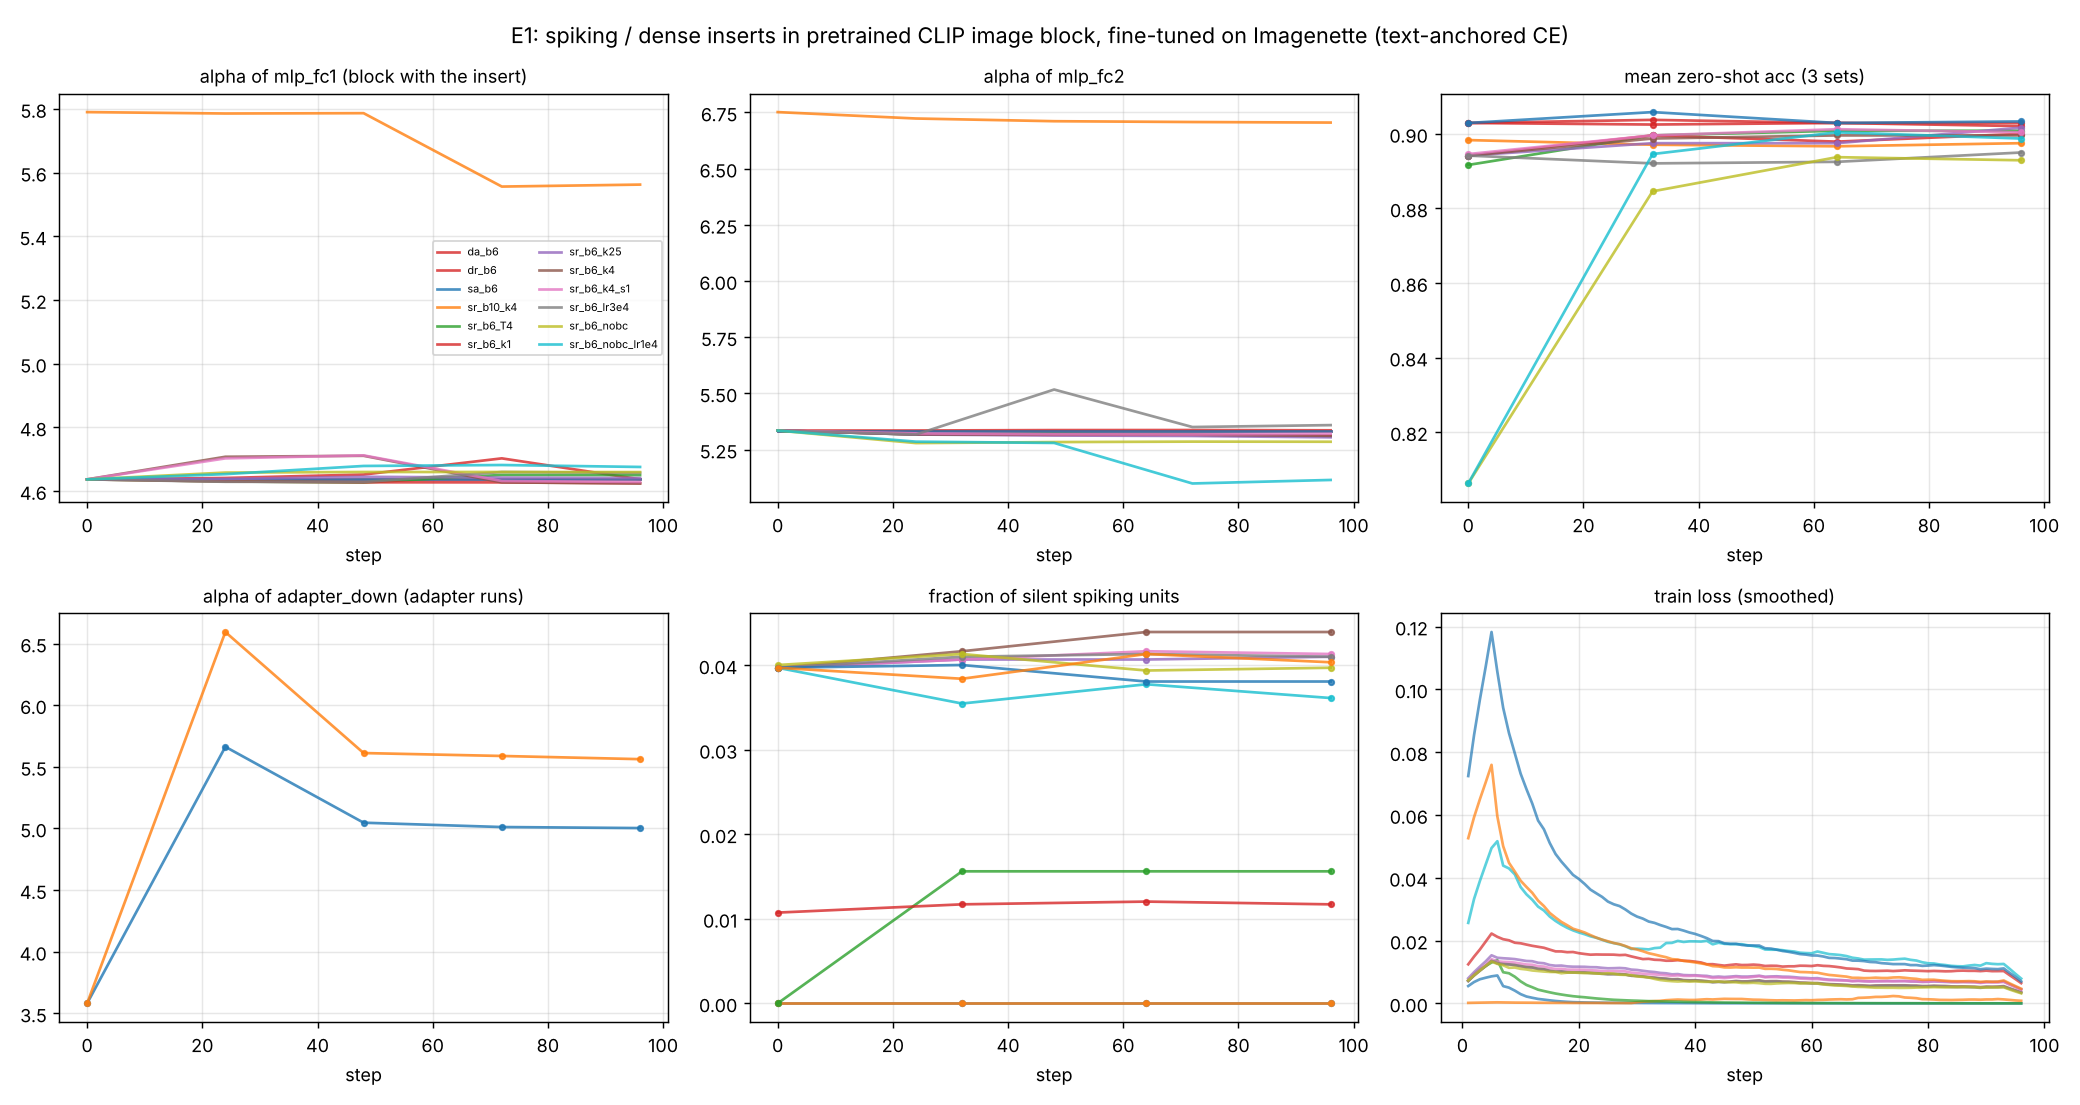
\includegraphics[width=\linewidth]{fig/e1_trajectories.png}
\caption{E1. Trajectories during three epochs of distillation fine-tuning after inserting a spiking (coloured) or dense (red) block into image block 6: $\alpha$ of fc1 / fc2, mean zero-shot accuracy, adapter $\alpha$, silent-unit fraction and training loss.}
\label{fig:e1}
\end{figure}
Every bias-corrected spiking replacement recovers from 0.892--0.895 to 0.900--0.902 (clean 0.903) and the uncorrected one from 0.806 to 0.893--0.899, while $\alpha_{\mathrm{fc1}}$ of the converted block moves by at most 0.04 and $\alpha_{\mathrm{fc2}}$ by at most 0.22 -- the same range as the dense twin that had nothing to repair (Fig.~\ref{fig:e1}). The repair is carried by small weight changes that do not touch the power-law tail of a $3072\times768$ matrix trained for 32 epochs on 400M pairs, so a within-run correlation between the block's $\alpha$ and the metric is meaningless (it flips sign across seeds on $\alpha$ changes of 0.01). Neither the surrogate slope ($k_{\mathrm{sg}}\in\{1,4,25\}$: $\alpha_{\mathrm{fc1}}$ 4.62, 4.62, 4.64, recovery 0.900--0.902), the time budget ($T\in\{4,8\}$), the seed, nor a $10\times$ larger learning rate creates dynamic range in $\alpha$. This is the opposite of the small-MLP result, where fc1 $\alpha$ rose monotonically with the slope ($1.60\to1.99$): the slope shapes a layer learned \emph{through} the spikes, not one that is nudged. The signals that do track the repair are the distillation loss and the firing statistics (silent fraction constant at 3.8--4.4\,\% in block 6, 1.2\,\% in block 10; no dead-unit growth). Zero-initialised adapters under distillation are a null task: accuracy is unchanged and the $\alpha$ of the random down-projection \emph{rises} from 3.6 to 5.0--5.6, the signature of an insert that is not needed; adapters under a learning objective are E3.
\subsection{E2b: cumulative conversion order}
\begin{figure}[t]
\centering
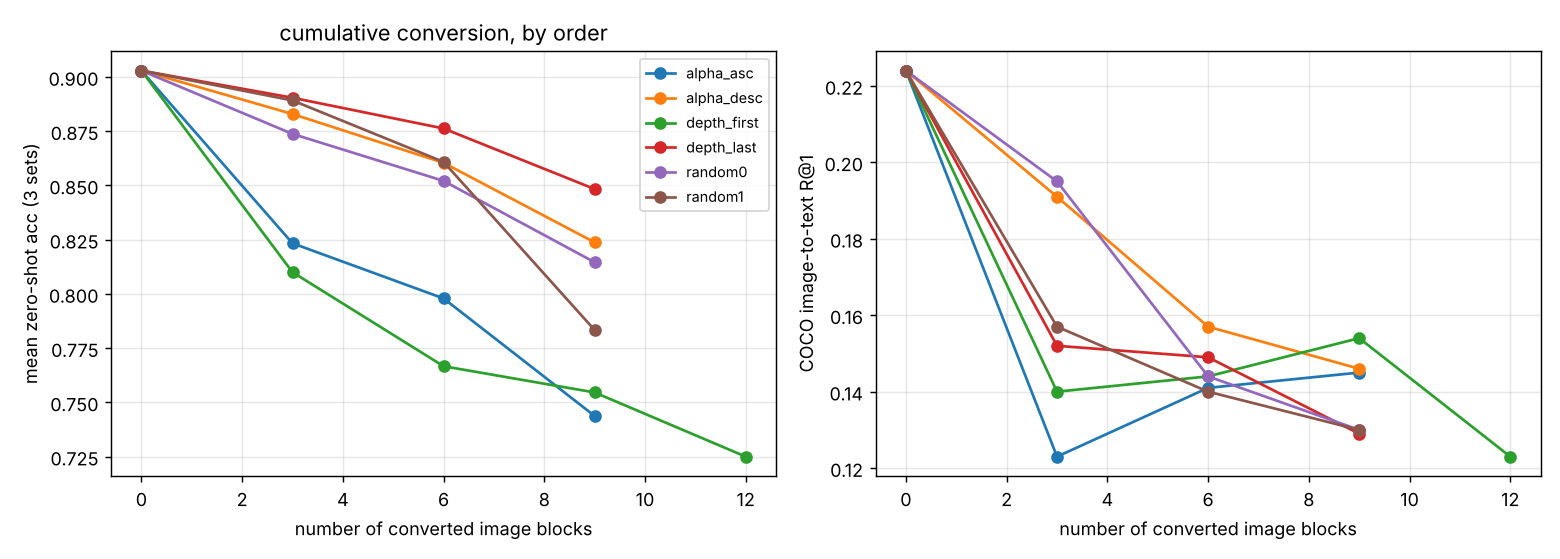
\includegraphics[width=\linewidth]{fig/e2b_orders.png}
\caption{E2b. Mean zero-shot accuracy (left) and COCO R@1 (right) after converting 3, 6, 9 or 12 image-block MLPs in six orders, conversion only (per-channel thresholds, bias correction, $T{=}8$, sequential calibration).}
\label{fig:e2b}
\end{figure}
Figure~\ref{fig:e2b} contradicts H2 at every fraction: converting the blocks whose MLP $\alpha$ is closest to 2 first costs 8.0 / 10.5 / 15.9 points at 3 / 6 / 9 blocks, the worst or second-worst of the six orders, while its reverse costs 2.0 / 4.3 / 7.9 and depth-last 1.3 / 2.7 / 5.5; the random orders rank by how many early blocks they contain. Damage compounds super-additively when early blocks are converted (closest-to-2 at 9 blocks: 15.9 against a sum of single-block drops of 9.1; depth-first 13.6 vs 6.9 at 6) and sub-additively when late blocks are (depth-last 5.5 vs 6.5), so sequential calibration recovers part of the loss when the converted blocks come late. All twelve MLPs convert at a cost of 17.8 points without fine-tuning (0.903 $\to$ 0.725). Retrieval does not follow the classification ranking: R@1 after three late blocks (0.15--0.19) is as damaged as after three early ones (0.12--0.14).
\subsection{E3: adapters on frozen embeddings}
\begin{table}[t]
\centering
\small
\begin{tabular}{lccccc}
\toprule
 & MLP & MLP & L3 & L3 spike & L3 spike \\
setting & dense & spike & dense & memory & rate \\
\midrule
Pets 16-shot acc & .854 & .842 & .729 & .744 & .763 \\
\quad transfer retained & .927 & .926 & .245 & .169 & .165 \\
Pets full acc & .867 & .852 & .809 & .849 & .848 \\
\quad transfer / COCO R@1 & .875/.204 & .886/.087 & .179/.049 & .447/.149 & .404/.128 \\
Imagenette 16-shot acc & .982 & .984 & .956 & .977 & .977 \\
$\alpha$ first matrix (Pets full) & 1.85 & 2.09 & 5.34 & 2.75 & 2.74 \\
$\alpha$ output matrix (Pets full) & 1.35 & 1.41 & 1.51 & 1.54 & 1.55 \\
\bottomrule
\end{tabular}
\caption{E3: residual adapters on frozen CLIP image embeddings, mean over 3 seeds (std $\le$ 0.02). Zero-shot: Pets 0.834, Imagenette 0.985. ``Transfer retained'' is the mean zero-shot accuracy on the two other classification sets after adaptation.}
\label{tab:e3}
\end{table}
Table~\ref{tab:e3} summarises 45 runs. A spiking MLP adapter matches its dense twin on classification within 1--1.5 points and keeps transfer, but halves retrieval R@1 in the full-shot setting: the rate-coded bottleneck preserves the class decision and not the fine-grained embedding geometry. The L3 lookup adapters as designed are harmful: routing by a $k$-means token applies a training-set-specific offset to every input, so transfer collapses and the 16-shot runs end below zero-shot. The spiking memory is consistently better than the dense L3 (full-shot 0.849 vs 0.809, transfer 0.45 vs 0.18) because the threshold-selected, count-normalised read-out is a sparser perturbation than the softmax-weighted one (memory firing fraction 0.17--0.35).

$\alpha$ behaves as a diagnostic in both directions. The first matrix of a working adapter converges to $\alpha \approx 2$ with the full Pets set (dense 1.85, spiking 2.09), stays at 2.7--2.9 with 16 shots and at 4.1--4.5 on the easy Imagenette task where nothing needs to be learned; across the 18 MLP-adapter runs its $\alpha$ correlates with the accuracy gain over zero-shot at Spearman $-0.73$ ($p=0.001$). The output matrices sit at $\alpha$ 1.35--1.7 in every run, and across all 45 runs the output-matrix $\alpha$ correlates with transfer retained at Spearman $-0.78$ ($p<10^{-4}$): the adapters whose output matrix became most heavy-tailed are the ones that over-specialised. The H3 prediction that the spiking memory's mixing layers settle at 2.0--2.2 is directionally right (spiking $W_{\mathrm{up}}$ 2.4--2.9 vs dense 4--5) but numerically wrong.

\section{Conclusion}
On a pretrained CLIP ViT-B/32, HTSR $\alpha$ is a useful diagnostic of \emph{fresh} matrices (an adapter that learns converges to $\alpha\approx2$, an unneeded one drifts up, an over-specialised output matrix drops below 2) but not a certificate for the repair of a \emph{pretrained} block, whose spectrum is inert under the fine-tuning that restores accuracy. As a selection signal its sign is the opposite of the hypothesis: low-$\alpha$ blocks carry the signal and are the most expensive to convert, so ``farthest from 2 first'' (in practice: late blocks first) is the rule, and damage compounds when early blocks are converted. The practical enablers are not spectral at all: per-channel thresholds and a bias correction for the GELU negative lobe make single-block conversion nearly free and full MLP conversion a 17.8-point loss before any training, and distillation to the clean embedding repairs an inserted block in one epoch where a task loss does not.
